% !TEX encoding = UTF-8 Unicode
\documentclass[a4paper]{article}

\usepackage{color}
\usepackage{url}
\usepackage[T2A]{fontenc} % enable Cyrillic fonts
\usepackage[utf8]{inputenc} % make weird characters work
\usepackage{graphicx}
\usepackage[table,xcdraw]{xcolor}
\graphicspath{ {./Slike/} }

\usepackage[english,serbian]{babel}
%\usepackage[english,serbianc]{babel} %ukljuciti babel sa ovim opcijama, umesto gornjim, ukoliko se koristi cirilica

\usepackage[unicode]{hyperref}
\hypersetup{colorlinks,citecolor=green,filecolor=green,linkcolor=blue,urlcolor=blue}

\usepackage{listings}

%\newtheorem{primer}{Пример}[section] %ćirilični primer
\newtheorem{primer}{Primer}[section]


\definecolor{mygreen}{rgb}{0,0.6,0}
\definecolor{mygray}{rgb}{0.5,0.5,0.5}
\definecolor{mymauve}{rgb}{0.58,0,0.82}

\lstset{ 
  backgroundcolor=\color{white},   % choose the background color; you must add \usepackage{color} or \usepackage{xcolor}; should come as last argument
  basicstyle=\scriptsize\ttfamily,        % the size of the fonts that are used for the code
  breakatwhitespace=false,         % sets if automatic breaks should only happen at whitespace
  breaklines=true,                 % sets automatic line breaking
  captionpos=b,                    % sets the caption-position to bottom
  commentstyle=\color{mygreen},    % comment style
  deletekeywords={...},            % if you want to delete keywords from the given language
  escapeinside={\%*}{*)},          % if you want to add LaTeX within your code
  extendedchars=true,              % lets you use non-ASCII characters; for 8-bits encodings only, does not work with UTF-8
  firstnumber=1,                % start line enumeration with line 1000
  frame=single,	                   % adds a frame around the code
  keepspaces=true,                 % keeps spaces in text, useful for keeping indentation of code (possibly needs columns=flexible)
  keywordstyle=\color{blue},       % keyword style
  language=C++,                 % the language of the code
  morekeywords={*,...},            % if you want to add more keywords to the set
  numbers=left,                    % where to put the line-numbers; possible values are (none, left, right)
  numbersep=5pt,                   % how far the line-numbers are from the code
  numberstyle=\tiny\color{mygray}, % the style that is used for the line-numbers
  rulecolor=\color{black},         % if not set, the frame-color may be changed on line-breaks within not-black text (e.g. comments (green here))
  showspaces=false,                % show spaces everywhere adding particular underscores; it overrides 'showstringspaces'
  showstringspaces=false,          % underline spaces within strings only
  showtabs=false,                  % show tabs within strings adding particular underscores
  stepnumber=1,                    % the step between two line-numbers. If it's 1, each line will be numbered
  stringstyle=\color{mymauve},     % string literal style
  tabsize=2,	                   % sets default tabsize to 2 spaces
  title=\lstname                   % show the filename of files included with \lstinputlisting; also try caption instead of title
}

\addtocontents{toc}{\setcounter{tocdepth}{1}} 

\begin{document}

\title{GNU GDB debager\\ \small{Seminarski rad u okviru kursa\\Metodologija stručnog i naučnog rada\\ Matematički fakultet}}

\author{Kristina Pantelić 91/2016 
Ivana Cvetkoski 65/2016\\
Bojana Ristanović 45/2016 
Nikola Stamenić 177/2016\\ 
\\kristinapantelic@gmail.com  
ivana.cvetkoski@gmail.com\\
trećeg 
mi16177@alas.matf.bg.ac.rs}

%\date{9.~april 2015.}

\maketitle

\abstract{
sazetak}

\tableofcontents

\newpage

\section{Uvod}
\label{sec:uvod}

Može se reći da je sastavni deo pisanja programa njegovo
debagovanje, jer je pojava bagova gotovo neizbežna. Greške nisu uvek
loše za pojedinca. Uz pozitivan stav možemo da uvidimo prednosti
poput poboljšanog razumevanja samog rada programa, učenja o sebi
tj. kakve greške najčešće pravimo, sticanja uvida o čitljivosti i
kvalitetu sopstvenog koda. Imajući u vidu potrebe i raznolikost
zadataka koje programer ima, teško je preceniti značaj odgovarajuće
alatne podrške za programere. Na samom početku ovog rada
upoznaćemo se sa bagovima i debagovanjem, a u daljem tekstu ćemo
detaljnije opisati specifičnosti debagera GDB, kako i u kojim
okruženjima se koristi, kao i poređenje sa drugim debagerima.

\section{Bag}
\label{sec:bag}
Čak i kada je program sintaksno ispravan, to još uvek ne znači da on i radi ono za šta je napisan. 
U tom slučaju program sadrži greške logičke prirode, tj. programer je tokom pisanja programa 
pogrešno protumačio značenje (semantiku) pojedinih naredbi koje je napisao. Otkrivanje i ispravljanje
semantičkih grešaka je daleko teže od otkrivanja i ispravljanja sintaksnih grešaka. 
Popularni naziv za semantičku grešku u programu je bag (\textit{eng.} bug).

Propust (greška, bag) u razvoju softvera je sve ono što stvara probleme u funkcionisanju softvera 
kao završnog proizvoda. "Bag predstavlja sve ono što ima za posledicu da se softver ne ponaša u 
skladu sa specifikacijom ili očekivanjem korisnika."

\vspace{4mm}

Jedna od uobičajenih klasifikacija bagova je prema načinu ispoljavanja:
\begin{enumerate}
\item nekonzistentnosti u korisničkom interfejsu
\item neispunjena očekivanja
\item slabe performanse
\item padovi sistema (program) ili oštećenja podataka
\end{enumerate}

\vspace{4mm}

Razlozi za greške uglavnom spadaju u sledeće kategorije procesa:
\begin{enumerate}
\item Kratki ili nemogući rokovi
\item Pristup „Prvo kodiraj, razmišljaj kasnije“
\item Pogrešno shvaćeni zahtevi
\item Neznanje inženjera ili nepravilna obuka
\item Nedostatak posvećenosti kvalitetu
\end{enumerate}


\section{Debagovanje}	
\label{sec:debagovanje}

Debagovanje (\textit{eng.} debugging) je proces pronalaženja i otklanjanja grešaka ili 
nedostataka koji sprečavaju tačnu operaciju računarskog softvera ili sistema. Kvar se 
obično otkriva jer se program neočekivano ponaša. Da bi se pronašao uzrok kvara, 
ključno je objasniti zašto dolazi do takog ponašanja. Debagovanje ima tendenciju da 
bude teže kada su različiti podsistemi čvrsto povezani, pošto promene u jednom mogu da 
prouzrokuju nastanak bagova u drugom.

\vspace{4mm}

"Otklanjanje grešaka je dvostruko teže nego pisanje koda. Stoga, ako napišete kod što 
je pametnije moguće,po definiciji, niste dovoljno pametni da ga ispravite."\\
\hspace*{0pt}\hfill\textit{-Brian V. Kernighan}

\vspace{4mm}
Debagovanje se sastoji iz četiri koraka:
\begin{enumerate}
\item uočavanje da postoji greška
\item razumevanje greške
\item lociranje greške
\item ispravljanje greške
\end{enumerate}

\vspace{4mm}

Obično je najteži deo posla ispravno razumevanje i tačno lociranje greške. Jednom kada 
se greška locira, njeno ispravljanje u većini slučajeva ne predstavlja poseban problem.

Testiranje je metod koji smanjuje verovatnoću nastajanja grešaka.
Otklanjanje grešaka se razlikuje od testiranja. Debagovanje počinje
nakon što je u softveru utvrđena greška, dok se testiranje koristi da bi
se osiguralo da je program tačan.

Debagovanje je jedan od najkreativnijih i najintelektualnijih aspekata programiranja, 
ali može biti i jedan od najstrašnijih. Odlike koje poseduju uspešni debageri su 
kreativnost, logičko zaključivanje, odlučnost, kao i razmišljanje na drugačiji način.
Veština debagovanja programera može biti bitan faktor u debagovanju, ali težina 
debagovanja softvera najviše varira zbog složenosti sistema, takođe zavisi, u određenoj 
meri, i od programskog jezika koji se koristi kao i dostupnih alata, kao što su 
debageri. 

Klasično debagovanje se zasniva na tehnici praćenja koda korišćenjem funkcije za ispis, tako što 
ispisujemo vrednosti promenljivih. Pre svega, ovaj način podrazumeva konstantno pozivanje funkcije za 
ispis, rekompajliranje i pokretanje programa, analize dobijenog izlaza i konačno uklanjanje 
poziva funkcije za ispis kada uspemo da popravimo bag. Navedeni koraci se ponavljaju svaki put 
kada otkrijemo novi bag. Ovaj način debagovanja oduzima previše vremena, stvara umor i najvažnije
odvlači pažnju od pravog zadatka.

Suprotno tome, sa grafičkim alatima za uklanjanje bagova sve što moramo da uradimo kako bismo 
ispitali vrednost promenljive je da pomerimo miš do instance te promenljive u kodu i biće
prikazana njena trenutna vrednost. Pored ovoga, debageri pružaju još dosta razloga da ih koristimo.

\subsection{Debager}
\label{subsec:debager}
Debager ili alat za debagovanje je računarski program koji se koristi da testira i 
debaguje druge programe ("meta" program), dajući mogućnost da se nezavisno 
pokrene izabrana grupa instrukcija (simulator grupe instrukcija).
To je alat koji omogućuje programeru da prati izvršavanje 
programa, da ga zaustavi, restartuje, postavi mesta prekida, i da
izmeni vrednosti u memoriji. Simulator grupe instrukcijase zaustavlja
na određenim tačkama programa ukoliko su određeni uslovi ispunjeni.
Obično se programi koji se prevode u režimu za debagovanje
sporije izvršavaju nego kada se isti program izvršava u normalnom režimu rada čak i ako je 
u pitanju rad na istom procesoru. \cite{debugger} Kada program usled baga ili netačnog podatka ne može da 
nastavi normalno sa radom, debager pokazuje lokaciju problema u originalnom kodu, takođe
debager nam omogućava da postavimo tačke posmatranja koje nam
mogu reći u kom trenutku tokom izvođenja programa vrednost
određene promenljive dobija sumnjivu vrednost, omogućava nam da
pratimo izvršavanje programa, da ga zaustavimo, restartujemo,
postavimo mesta prekida, i da izmenimo vrednosti u memoriji. 

\section{GNU debager (GDB)}
\label{sec:GDB}
GNU debager (\textit{eng.} GNU Debugger) kog često srećemo pod nazivom GDB je alat koji služi za pronalaženje 
i otklanjanje grešaka tj. debagovanje. Originalno ga je razvijao Ričard Stalman 1986. godine, kao i mnoge druge programe za GNU sistem\cite{gdb}. Danas održavanjem upravlja GDB upravni odbor koga je formirala Fondacija 
slobodnog softvera (\textit{eng.} Free Software Foundation).
GDB je pisan na programskom jeziku C i standardni je debager za GNU operativni sistem. 
Međutim, njegova upotreba nije isključivo ograničena na GNU operativni sistem. To je prenosivi debager
koji radi na mnogim Uniksolikim (eng. \textit{unixlike}) operativnim sistemima ali i na Microsoft Windows operativnim 
sistemima i Mac OS X. Koristi se za mnoge programske jezike, uključujući
Adu, C, C++, Objective-C, Free Pascal, Fortran, Javu.
Poslednja realizovana verzija alata GNU GDB u vreme pisanje ovog rada je 9.1. \cite{sourceware}

GDB je konzolni alat (pokreće se iz konzolne linije). Međutim, zbog popularnosti grafičkih korisničkih interfejsa
(\textit{eng.} GUI) razvijen je veliki broj debagera sa grafičkim korisničkim okruženjem za Unix sisteme\cite{art_debugging}. 
Jedan od najpoznatijih debagera sa GUI-em je DDD, koji podržava grafički prikaz za više debagera, među kojima je
GDB, a pored njega i DBX, WDB, Ladebug, JDB, XDB. Sam DDD se više ne razvija, od 2011-e, zaključno sa verzijom 3.3.12. \cite{GNUOrg}
Pored DDD-a, KDbg je još jedan vid grafičkog okruženja za GDB koji se više ne razvija. KDbg je bio namenjen
Linux operativnim sistemima sa KDE grafičkim okruženjem. Jedan od trenutno aktuelnih grafičkig interfejsa jeste
gdbgui, o kojem će više reči biti u delu \ref{subsec:gdbgui}.

Sa druge strane, danas je sve veća upotreba integrisanih razvojnih okruženja (\textit{eng.} IDE),
koji predstavlja više od alata za debagovanje. IDE obuhvata editor, alat za izgradnju koda, debager i druga 
razvojna pomagala. Jedan od najpoznatijih IDE okruženja koje koristi GDB debager je Eclipse sistem,
a pored njega prisutan je i u CLion-u, QT Creatoru-u, Code::Blocks-u\cite{sourceware}.
Korišćenje GDB-a kroz QT Creator će biti podrobnije objašnjeno u delu \ref{subsec:QT}

Jedna od specifičnosti GNU GDB debagera, pored svoje standardne namene, jeste da omogućava i 
pronalaženje, analiziranje i otklanjanje grešaka u programima koji se izvršavaju na računarima drugih 
arhitektura (udaljeno debagovanje)\cite{master_rad}.

\subsection{Osnovne operacije GDB-a}
\label{subsec:debager_operacije}

GDB komanda \textbf{run}, pokreće izvršavanje programa od prve linije izvornog koda.
Izvršavanje programa teče do trenutka dok GDB ne pauzira izvršavanje programa. 
Razlog pauziranja izvršavanja programa može biti na programskoj ili programerskoj strani.
Pod programskom stranom podrazumeva se pauziranje izvršavanja programa zbog greške 
nastale u izvršavanju. Pod programerskom stranom podrazumeva se pauziranje izvršavanja 
programa na mestima specifikovanim od strane programera kako bi se mogle ispitati 
vrednosti promenljivih u cilju otkrivanja grešaka.

\subsubsection{Metode upravljanja debagovanjem u GDB-u}
\label{subsec:gdb_metode}

Naime, da bi se sam GDB koristio na određenom programu, neophodno je isti kompajlirati 
na određen način. Za programske jezike C i C++ to je zastavicom \textit{-g}, odnosno
\textit{gcc program.c -g -o program} za C, dok je za C++ \textit{g++ program.cpp -g -o program}.\\
Jedna jako korisna opcija je navođenje \textit{--tui} zastavice pri pokretanju samog debagera. 
Korisna je iz razloga što korisnik dobija izvorni kod programa koji debaguje, što dalje olakšava posao postavljanja
tačaka prekida i eventualno uočavanje nekih od grešaka\cite{oReilly}.\\
Neke od metoda kojima programer može upravljati GDB debagerom radi debagovanja programa:\cite{art_debugging}
\begin{enumerate}
\item Tačke zaustavljanja (\textit{eng.} breakpoints) \\
Komandom \textbf{break}, uz koju se navodi broj linije na kojoj GDB treba da pauzira izvršavanje, 
uvodi se nova tačka zaustavljanja. Cilj zaustavljanja izvršavanja programa je ispitivanje vrednosti
promenljivih u programu kako bi se otkrila greška.
\item Pojedinačni koraci (\textit{eng.} single-stepping)\\
GDB komanda \textbf{next} omogućava izvršavanje jedne po jedne linije programa. 
Nakon jedne izvršene linije koda, GDB pravi pauzu u izvršavanju programa dok se ponovo ne 
pozove komanda \textbf{next}. Komanda \textbf{step} je slična prethodno pomenutoj 
komandi ali drugačija. Razlika je u tome što ukoliko je naredna naredba za izvršavanje funkcija, 
komandom \textbf{step} se ulazi u funkciju i korak po korak prolazi kroz nju. Sa druge strane 
komanda \textbf{next} izvršava čitavu funkciju u jednom koraku, vraća njenu povratnu 
vrednost i zaustavlja se na liniji u kodu nakon izvršene funkcije.
\item Nastavi rad (\textit{eng.} resume operation)\\
GDB komandom \textbf{continue} nastavlja se izvršavanje programa do naredne tačke zaustavljanja. 
\item Privremene tačke zaustavljanja (\textit{eng.} temporary breakpoints)\\
GDB komandom \textbf{tbreak} postavlja se tačka zaustavljanja u programu koja će važiti 
sve do njenog prvog dostizanja u izvršavanju programa. Nakon njenog prvog dostizanja, 
ta tačka zaustavljanja prestaje da važi. 
\end{enumerate}

\subsubsection{Kretanje kroz stek pozive naviše i naniže}
\label{subsec:debager_stek}

S obzirom da su pozivi funkcija smešteni u stek okvirima, jer se u samim okvirima nalaze vrednosti
lokalnih promenljivih, parametri funkcije kao i memorisana lokacija u programu odakle je funkcija pozvana, 
potrebne su nam funkcionalnosti uz pomoć kojih možemo da se "šetamo" kroz njih.
To uspevamo narednim komandama: \\
\indent Pozivanjem GDB komande \textbf{frame}, okviri na steku se numerišu od nule - počevši
od vrha steka. \newline 
\indent GDB komanda \textbf{up} vodi do narednog roditeljskog stek frejma, dok komanda \textbf{down} 
vodi u suprotnom smeru. Navedene operacije mogu biti veoma korisne, jer vrednosti lokalnih 
promenljivih u nekim od ranijih poziva mogu dati rešenje o tome šta je tačno izazvalo bag\cite{art_debugging}. 
GDB komanda \textbf{backtrace} pokazuje ceo stek tj. celu kolekciju stek frejmova koja trenutno postoji na steku.

Neke od najbitnijih komandi GDB-a date su u tabeli \ref{tab:tabelaKonzola}, dok se više informacija
može naći na \textit{http://www.yolinux.com/TUTORIALS/\\GDB-Commands.html\#GDB\_COMMAND\_LINE\_ARGS},
kao i u MAN stranama Linux operativnih sistema.

\begin{table}[!h!]
\begin{center}
\caption{Tabela nekih od najbitnijih komandi.}
\begin{tabular}{|p{4cm}|p{6cm}|} \hline
Komanda & Značenje\\ \hline
help <klasa|komanda|all> & Izlistavanje pomoći za klasu komandi, samu komandu ili sve klase komandi\\ \hline
run & Pokretanje samog programa, sa svim navedenim tačkama prekida \\ \hline
appropos \textit{reč} & Pretraga komande vezane za datu reč\\ \hline
info args & Izlistavanje argumenata komandne linije \\ \hline
info breakpoints & Izlistavanje tačaka prekida \\ \hline
info registers & Izlistavanje registara u upotrebi \\ \hline
info threads & Izlistavanje niti koje program koristi \\ \hline
break +|- broj-linija & Postavljanje tačke prekida za dati broj linija od trenutne pozicije pri prekidu \\ \hline
delete & Brisanje svih tačaka prekida \\ \hline
delete broj-tačke-prekida & Brisanje tačke prekida sa određenim brojem \\ \hline
disable broj-tačke-prekida | raspon & Isključivanje tačke prekida sa datim brojem ili više tačaka u nekom rasponu \\ \hline
enable broj-tačke-prekida & Uključivanje tačke prekida sa određenim brojem \\ \hline
continue | c & Nastavak izvršavanja do naredne tačke prekida \\ \hline
finish & Dovršavanje izvršavanje započete funkcije \\ \hline
step <broj-koraka> & Prelazak na narednu liniju koda, ili liniju za određen broj koraka udaljenu \\ \hline
next <broj-koraka> & Izvršavanje naredne linije koda, ili narednih <broj-koraka> linija koda \\ \hline
where & Prikaz trenutne pozicije u kodu, broj linije \\ \hline
backtrace & Prikaz trenutne pozicije, ime funkcije, kojim putem se došlo do tog stanja\\ \hline
<up|down><broj-okvira> & Pomeraj gore ili dule kroz stek okvire, za onoliko okvira koliko zadamo, ili jedan ako ne navedemo ništa \\ \hline
\end{tabular}
\label{tab:tabelaKonzola}
\end{center}
\end{table}

\subsubsection{Tačke zaustavljanja}
\label{subsec:gdbtackezaustavljanja}

Postoje tri razloga zbog kojih GDB može pauzirati izvršavanje programa:\cite{art_debugging}
\begin{enumerate}
\item Tačka zaustavljanja (\textit{eng.} breakpoint) \\
GDB pauzira izvršavanje programa kada se stigne do naznačenog mesta u programu.
\item Tačka nadgledanja (\textit{eng.} watchpoint) \\ 
GDB pauzira izvršavanje programa kada se promeni vrednost memorijske lokacije koju programer želi da prati.
\item Tačka hvatanja (\textit{eng.} catchpoint) \\
GDB pauzira izvršavanje programa kada se određeni događaj desi.
\end{enumerate}
U dokumentaciji ova tri mehanizma se zajedničkim imenom nazivaju tačke zaustavljanja. 

\subsubsection{Udaljeno debagovanje}
\label{subsec:gdb_udaljeno}

GDB pruža mogućnost udaljenog debagovanja koji se koristi za debagovanje ugradnih uređaja, 
uređaja na kojima se neposredno debagovanje ne može izvršiti ili debagovanje jezgra operativnog sistema. 
Udaljeno debagovanje podrazumeva da se GDB izvršava na jednoj mašini, a program koji se debaguje na 
drugoj mašini.
Jedan način uspostavljanja komunikacije za debagovanje udaljenog uređaja je kreiranje udaljenog posrednika koji je specifičan za konkretnu arhitekturu računara koji se debaguje. Udaljen posrednik je programski kod koji se izvršava na udaljenom uređaju i omogućava komunikaciju sa GDB-om. Sprecifičnost ovog načina komunikacije je neophodnost pravljenja udaljenog posrednika pri svakom debagovanju. 
Opisani koncept koristi KGDB za debagovanje Linux jezgra na nivou izvornog koda. Velika prednost KGDB-a 
je u tome što programeri koji razvijaju jezgro mogu debagovati jezgro na sličan način kao što se 
debaguje bilo koja druga programska aplikacija. Moguće je postavljati tačke zaustavljanja u kodu jezgra, 
prolaziti korak po korak kroz kod, ispitivati vrednosti promenljivih.\cite{kgd}

Alternativno, može se koristiti GNU GDB server (\textit{eng.} gdbserver) za udaljeno debagovanje 
programa bez potrebe da se bilo šta menja na obe strane komunikacije. GDBserver nije u potpunosti 
zamena za udaljene posrednike, jer nameće ograničenje da operativni sistemi klijenta i servera 
moraju biti isti. Zapravo, sistem koji pokreće GDBserver, da bi se povezao na udaljeni GNU debager, 
takođe mora lokalno pokrenuti GNU debager. Dobra strana je da GDBserver ne zahteva mnogo 
resursa na udaljenom računaru, jer se ponaša kao omotač programa koji se debaguje. 
Takođe, gdbserver je portabilniji pa je rad sa GDBserverom na novom uređaju brže nego u drugom slučaju. 

Način debagovanja GDBserverom sastoji se od klijentske strane koja traži usluge i serverske strane 
koja usluge i resurse nudi. U udaljenom debagovanju klijent predstavlja korisnički računar sa koga se 
debagovanje izvršava ka udaljenom računaru. Uz pomoć odgovarajućih protokola klijent se povezuje 
sa GDBserverom pokrenutim na udaljenom računaru\cite{master_rad}. 


% \section{Upotreba GDB-a}
% \label{sec:upotreba}
% 
% GNU Debugger je kao i većina GNU alata prvobitno bio namenjen za rad iz konzole. Kako je vreme prolazilo, javila se potreba za 
% grafičkim interfejsom kako bi se olakšao rad programera pri debagovanju. Tokom vremena javljala su se mnoga rešenja, kako
% samostalni grafički interfejsi, tako i razvojna okruženja koja koriste GDB kao svoj debager. Neka od grafičkih rešenja su
% \textbf{gdbgui}, \textbf{KDbg}, \textbf{CGDB}, dok su \textbf{CLion}, \textbf{Qt Creator}, \textbf{Code::Blocks} neka 
% od razvojnih okruženja koja podržavaju GDB\cite{sourceware}. Pojedini gorepomenuti alati će podrobnije biti opisani u daljem tekstu, kroz neki 
% vid upotrebe samih alata.


% \subsection{GDB iz konzole}
% \label{subsec:konzola}
% 
% Rad iz konzole možda nije previše popularna disciplina, ali može biti od velikog značaja ukoliko se debaguje neki kraći kod za koji
% nema potrebe podizati čitavo grafičko okruženje ili ukoliko se radi na sistemima ograničene 
% memorije. \\
% Kako bi se sam GDB pustio u rad, neophodno je pokrenuti ga komandom \textit{gdb program}. Postoje i drugi načini
% pokretanja samog programa, a neki od njih su \textit{gdb -e program -c core-fajl} kako bi imali određeni fajl
% u koji bi se upisivala stanja programa ili \textit{gdb program --id-procesa} kako bi se povezali sa već pokrenutim procesom.
% Ono na šta mi obraćamo pažnju je prvi vid pokretanja. Jedna jako korisna opcija je navođenje \textit{--tui} zastavice pri pokretanju
% samog debagera. Korisna je iz razloga što korisnik dobija izvorni kod programa koji debaguje, što dalje olakšava posao postavljanja
% tačaka prekida i eventualno uočavanje nekih od grešaka\cite{oReilly}. Tabela \ref{tab:tabelaKonzola} prikazuje neke od najbitnijih komandi
% GDB-a, dok se skup svih može naći na adresi \textit{http://www.yolinux.com/TUTORIALS/\\GDB-Commands.html\#GDB\_COMMAND\_LINE\_ARGS}.
% 
% 
% \begin{table}[h!]
% \begin{center}
% \caption{Tabela nekih od najbitnijih komandi.}
% \begin{tabular}{|p{4cm}|p{6cm}|} \hline
% Komanda & Značenje\\ \hline
% help <klasa|komanda|all> & Izlistavanje pomoći za klasu komandi, samu komandu ili sve klase komandi\\ \hline
% run & Pokretanje samog programa, sa svim navedenim tačkama prekida \\ \hline
% appropos \textit{reč} & Pretraga komande vezane za datu reč\\ \hline
% info args & Izlistavanje argumenata komandne linije \\ \hline
% info breakpoints & Izlistavanje tačaka prekida \\ \hline
% info registers & Izlistavanje registara u upotrebi \\ \hline
% info threads & Izlistavanje niti koje program koristi \\ \hline
% break +|- broj-linija & Postavljanje tačke prekida za dati broj linija od trenutne pozicije pri prekidu \\ \hline
% delete & Brisanje svih tačaka prekida \\ \hline
% delete broj-tačke-prekida & Brisanje tačke prekida sa određenim brojem \\ \hline
% disable broj-tačke-prekida | raspon & Isključivanje tačke prekida sa datim brojem ili više tačaka u nekom rasponu \\ \hline
% enable broj-tačke-prekida & Uključivanje tačke prekida sa određenim brojem \\ \hline
% continue | c & Nastavak izvršavanja do naredne tačke prekida \\ \hline
% finish & Dovršavanje izvršavanje započete funkcije \\ \hline
% step <broj-koraka> & Prelazak na narednu liniju koda, ili liniju za određen broj koraka udaljenu \\ \hline
% next <broj-koraka> & Izvršavanje naredne linije koda, ili narednih <broj-koraka> linija koda \\ \hline
% where & Prikaz trenutne pozicije u kodu, broj linije \\ \hline
% backtrace & Prikaz trenutne pozicije, ime funkcije, kojim putem se došlo do tog stanja\\ \hline
% <up|down><broj-okvira> & Pomeraj gore ili dule kroz stek okvire, za onoliko okvira koliko zadamo, ili jedan ako ne navedemo ništa \\ \hline
% \end{tabular}
% \label{tab:tabelaKonzola}
% \end{center}
% \end{table}

\section{Upotreba GDB-a kroz grafički pristup}
\label{subsec:gui}


\subsection{Grafičko okruženje gdbgui}
\label{subsec:gdbgui}

Alat \textbf{gdbgui} je grafičko okruženje za GDB, koji radi na nivou internet pretraživača.
Program se pokreće naredbom \textit{gdbgui} u terminalu, dok za više informacija o samim komandama
programa se može dobiti naredbom \textit{gdbgui -\phantom{}-help}\cite{gdbgui}. Samo korišćenje alata može biti
identično kao i iz konzole, s obzirom da program sadrži terminal u sebi za ispis koji GDB inače vrši. Ono 
što olakšava posao, i prevashodno razlog postojanja gdbgui-a, je lakše upravljanje tačkama prekida,
lakši pregled informacija od značaja, kao i prikaz samog izvornog koda, koji se kod konzolnog korišćenja 
dobija zastavicom -\phantom{}-tui. \\
Grafičko okruženje je podeljeno u nekoliko celina.Najupečatljivija je celina u kojoj se nalazi učitani kod. 
U njoj se postavljaju tačke prekida, klikom kursora na broj linije, a na isti način i uklanjaju.
Sa desne strane se nalazi nekoliko padajućih menija, koji predstavljaju prikaz odredjenih informacija 
u datom trenutku vremena, tako se tu mogu naći informacije o niti u kojoj se nalazimo, lokalnim promenljivama, 
registrima i ostalo. Iznad ove dve celine, nalazi se deo za kontrolisanje programa. Sačinjen je od prostora
za unos putanje do programa, koji će debager koristiti, a on će biti učitan u program klikom na dugme 
\textit{Load Binary}. Sa desne strane se nalazi nekoliko dugmića za kontrolu izvršavanja programa.
Tako se tu nalaze naredbe za ponovno učitavanje programa, izvršavanje do naredne tačke prekida, obustavljanje
programa, prelazak na sledeću instrukciju, na sledeći poziv funkcije, vraćanja nazad iz funkcije, kao i prelazak
na sledeću mašinsku instrukciju sa ili bez poziva funkcije. Za one koji su navikli da rade iz konzole, tu se nalazi 
i terminal. Na slici \ref{fig:gdbgui} je prikazano kako sam program izgleda kako bi se opisano približilo korisniku.\\
Pokretanje debagovanja je, kao i kroz konzolu, komandom \textit{run}. Nadalje korisnik sam bira da li će 
upravljati debagerom kroz konzolu, uz pomoć komandi datih u tabeli \ref{tab:tabelaKonzola}, ili kroz grafički interfejs.

\begin{figure}[h!]
\begin{center}
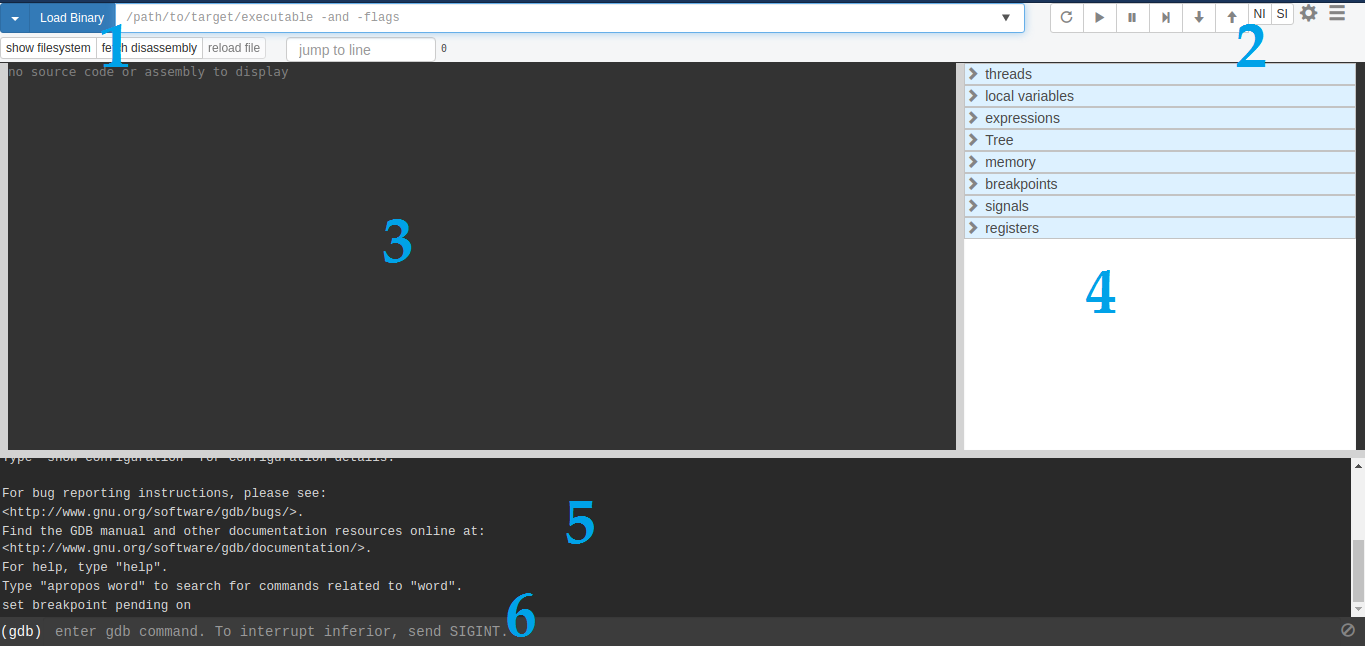
\includegraphics[scale=0.2]{gdbgui.png}
\end{center}
\caption{gdbgui: 1) Load Binary 2) Dugmići za kontrolu 3) Kod 4) Informacije o programu u tačkama prekida 5) Konzola 6) Promt}
\label{fig:gdbgui}
\end{figure}

\subsection{GDB u QT Creator razvojnom okruženju}
\label{subsec:QT}

Qt Creator je prenosivo radno okruženje koje je pravljeno prevashodno za Qt radni okvir (eng. \textit{framework}).
Kako je i sam Qt prenosiv kako među različitim vidovima arhitektura, tako i među samim sistemima, Qt Creator
mora da podržava različite prevodioce i debagere koje ti debageri koriste. Gnu Debager je podrazmevani debager
ukoliko se koristi GCC prevodilac na Linux-u, Unix-u, Windows-u u kombinaciji sa MinGW-om, dok je na macOS-u
eksperimentalne prirode. \cite{QT}
\\
Naime, sam Qt Creator podržava neki vid statičke analize koda, tako da u tok kreiranja koda programer može da 
uvidi neke moguće greške, kao što su nekompatibilnost tipova koji se koriste, izlaženje izvan granica niza (vektora) 
i sličnih koje su uočljive u tom momentu. Nažalost, dosta grešaka ostaje neprimećeno. Tu nam pomaže debager,
u ovom slučaju GDB, čija će upotreba, na nekom jednostavnijem nivou, biti prikazana kroz naredni kod. 

\begin{lstlisting}[caption={Primer jednostavnog programa za prikaz rada GDB-a u Qt Creator-u},frame=single, label=simple]
#include <iostream>
#include <vector>

using namespace std;

int main()
{

    string hello = "hello world";   \\prva tacka prekida
    cout << hello;                  \\druga tacka prekida

    auto vec = new vector<int>{1,2,3,4,5,6,7,8,9,10};

    for(size_t i = 0; i < vec->size(); i++)
        cout << vec->at(i);         \\treca tacka prekida

    delete vec;

    for(size_t i = 0; i < vec->size(); i++){
        cout << vec->at(i);         \\cetvrta tacka prekida
    }

}
\end{lstlisting}

Za početak, postavljanje tačaka prekida. Vrši se skoro isto kao i kod gdbgui-a, jedina je razlika što kod Qt Creator-a
se ne klikće na sam broj linije, već malo levo od broja, te se tu prikazuje kružić koji označava da je
tačka prekida postavljena. Ona se može onemogućiti/omogućiti ili uređivati desnim klikom na kružić i biranjem određene funkcionalnosti.
Slika \ref{fig:point_info} prikazuje informacije o samoj tački prekida kada se
kursorom pozicioniramo na dobijeni kružić. Tu imamo informacije o internom id-u tačke prekida, koji se dodeljuje
po redosledu postavljanja, ne po redosledu u kodu počevši od prve linije, stanje tačke prekida (\textit{Internal ID}),
stanje tačke prkida, odnosno da li je omogućena ili ne (\textit{State}), tip tačke prekida (\textit{Breakpoint Type}),
fajl u kojem se tačka prekida nalazi (\textit{Marker File}), broj linije u fajlu na kojoj se nalazi tačka prekida (\textit{Marker Line})
i broj koliko smo se puta zaustavili u toj tački prekida (\textit{Hit Count}).
Na samom vrhu slice se nalazi žuta strelica, naime ona se ne nalazi tu stalno, već samo u momentu kada je program 
zaustavljen u toj tački prekida i ispitujemo inormacije za tu tačku.

\begin{figure}[h!]
\begin{center}
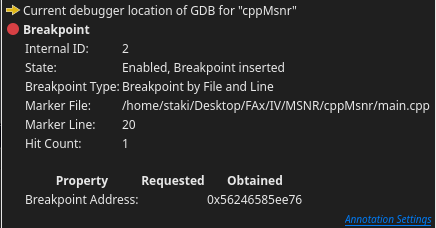
\includegraphics[scale=0.7]{breakpoint_info.png}
\end{center}
\caption{Informacije o jednoj tački prekida}
\label{fig:point_info}
\end{figure}

Prilikom dodavanja tačaka prekida, one se dodaju u listu svih tačaka prekida. Za ovako jedonstavan program to 
nije od krucijalnog značaja, dok kod kompleksijih programa može biti od velike pomoći. U samom spisku tačke
prekida mogu da se uređuju, omogućuju ili onemogućuju, kao i da se brišu iz spiska. Kako spisak izgleda, dato 
je slikom \ref{fig:points_list}.

\begin{figure}[h!]
\begin{center}
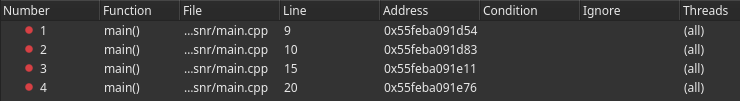
\includegraphics[scale=0.7]{breakpoints_list.png}
\end{center}
\caption{Spisak tački prekida i neke dodatne informacije o njima}
\label{fig:points_list}
\end{figure}

Kada smo postavili tačke prekida, vreme je da pokrenemo program u debag režimu. To se može postići na više načina,
najlakši od njih je klikom na "play" dugme u donjem levom uglu, sa nacrtanom bubom na sebi, moguće je i klikom na 
dugme \textbf{F5} na tastaturi, kao i odlaskom u meni \textbf{Debug->Start Debugging} \cite{QT}.
\\

Program pri izvršavanju staje na svaku od tačaka prekida i daje informacije o svim promenljivim iz tog dosega. 
Informacije o promenljivama u svakoj od tačaka prekida su date slikom \ref{fig:points_res}. 
Ono što primećujemo u tom delu je da GDB daje informacije o imenu promenljive, tipu promenljive i njenoj vrednosti, 
ukoliko ju je moguće koristiti, u suprotnom stoji poruka \textbf{\textit{<not accessible>}}. Ta poruka nam šalje
informaciju da tu promenljivu ne bi trebalo koristiti u tom delu koda. U našem primeru, u liniji 17 smo pokazivač "poništili" 
i on više nije validan, što nam četvrta tačka prekida i govori, ali u toj liniji pokušavamo da ispišemo vrednost prvog elementa
tog vektora. Ta greška je prouzrokovala \textbf{Segmentation Fault}, dok nam GDB izbacuje obaveštenje dato slikom \ref{fig:signals}.
Problem u ovom vidu ispisa jeste i što nema informacija gde se ta greška dogodila.

\begin{figure}[h!]
\begin{center}
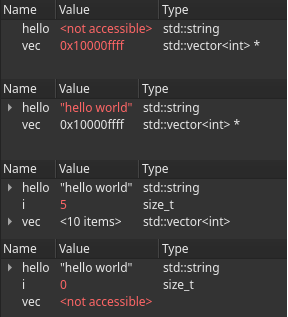
\includegraphics[scale=0.5]{breakpoints_res.png}
\end{center}
\caption{Informacije o promenljivama u tačkama prekida}
\label{fig:points_res}
\end{figure}


\begin{figure}[h!]
\begin{center}
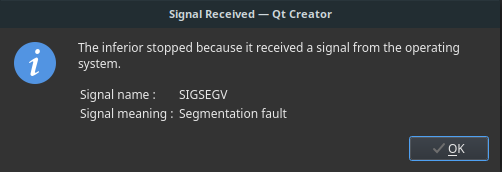
\includegraphics[scale=0.5]{signals.png}
\end{center}
\caption{Signal pri nepravilnom završavanju programa}
\label{fig:signals}
\end{figure}


\section{Poređenje sa drugim popularnim dibagerima}
\label{sec:poredjenje}
Danas je teško zamisliti da bismo mogli napraviti bilo koji značajan projekat bez korišćenja
naprednih alata za pronalaženje grešaka. Postoji mnogo dibagera koji se mogu koristit kako
na različitim operativnim sistemima tako i za različite programske jezike. 
Neke od stvari na koje treba obratiti paznju prilikom izbora dibagera:

\begin{enumerate}
\item Debagovanje u fazi razvoja \\
Dobar program za otklanjanje grešaka treba da podržava
programera u svakoj od sledećih faza uklanjanja grešaka:
primećivanje greške, pronalaženje uzroka, ispravljanje greške.
Potrebno je izabrati program koji nam omogućava da uvidimo kako
su naše promene uticale na ceo sistem.
\item Efikasno praćenje toka vrednost\\
Najvažniji faktor efikasnog lociranja uzroka greške predstavlja
razumevanje detalja i načina na koji kod funkcioniše. Svaki od
dibagera podražava programera u ovom zadatku na drugačiji način.
\item Debagovanje grešaka u višenitnim procesima\\
Savremene aplikacije su višenitni i višeprocesni sistemi. 
{\em Potraga za uzrokom greške u mnogim slučajevima liči na traženje igle u
plastu sena. Posebno višenitne aplikaje zahtevaju veliko znanje
programera o funkcionisanju celog sistema.\cite{tools} } Srećom, neki alati
omogućavaju pregledanje pojedinačnih niti.
\item Da li program za otklanjanje grešaka brzo i lako šalje detaljne informacije o otkrivenim greškama?
\end{enumerate}

\subsection{GDB i LLDB}
\label{subsec:lldb}
LLDB je program za otklanjanje grešaka koji se koristi u LLVM 
(\textit{eng.} Low Level Virtual Machine) projektima. To je besplatan softver sa 
otvorenim kodom (\textit{eng.} open source) pod licencom 
Univerziteta Ilionis / NCA Open Source Licence. Napravljen je kao 
skup komponenata za višekratnu upotrebu.

LLDB je napravljen od strane LLVM razvojne grupe dok je GDB 
realizacija GNU projekta. Druga razlika je u tome što je LLDB 
pisan u CPP-u, a GDB u C-u. Što se operativnih sistema tiče, LLDB 
radi na macOS i386 i x86-64, Linux-u,  FreeBSD-u, Windows-u, 
dok je GDB prenosiv program za otklanjanje gešaka koji radi na 
mnogim UNIX sistemima i Windows-u. Jedna od glavnih razlika 
između ova dva programa predstavljaju programski jezici u kojima 
se koriste. LLDB može biti koršćen da otkloni greške u C, Objective 
C i CPP programima, a GDB se može koristiti za jezike  Ada, C, 
CPP, Objective C, Pascal, FORTRAN i Go.

Iako je veliki deo komadi sličan, postoje razlike u nekim od 
najčešće korišćenih. Razlike su date u tabeli \ref{tab:tabela1}:


\begin{table}[h!]
\begin{center}
\caption{Razlike između GDB i LLDB komandi}
\begin{tabular}{|l|c|c|} \hline
                                                 & GDB            & LLDB                                                                  \\ \hline
\rowcolor[HTML]{C0C0C0} 
Pokretanje programa                              & run            & process launch                                                        \\
Prikaz vrednosti u registrima                    & info registers & registers read                                                        \\
\rowcolor[HTML]{C0C0C0} 
Prikaz tačaka prekida                            & info break     & breakpoint list                                                       \\
Izbrisi sve tačke prekida                        & delete         & breakpoint delete                                                     \\
\rowcolor[HTML]{C0C0C0} 
Izbriši tačku prekida označenu sa broj           & delete (broj)  & \multicolumn{1}{l|}{\cellcolor[HTML]{C0C0C0}breakpoint delete (broj)} \\
Prikaz vrednosti svih lokalnih promenljivih      & info locals    & frame variable                                                        \\
\rowcolor[HTML]{C0C0C0} 
Prikaz vrednosti lokalne promenljive prom        & p prom         & frame variable prom                                                   \\
Prikaz stanja steka za trenutnu nit              & bt             & thread backtrace                                                      \\
\rowcolor[HTML]{C0C0C0} 
Izlistaj glavnu izvršnu biblioteku i sve zavisne & info shared    & image list                                                            \\ \hline
\end{tabular}
\label{tab:tabela1}
\end{center}
\end{table}

\subsection{GDB i VALGRIND}
\label{subsec:valgrind}
Valgrind je programski alat za pronalaženje grešaka u memoriji, otkrivanja curenja memorije i 
profajliranje. To je besplatan softver, otvorenog koda koji je pod GNU General Public licencom. 
Uz njega dolazi nekoliko alata. Osnovni i njaviše korišćen je Memcheck, koji može da otkrije i  
prijavi sledeće vrste grešaka u memoriji: korišćenje neinicijalizovane memorije, čitanje/pisanje u 
memoriju nakoj što je oslobođena, čitanje/pisanje na kraj alociranog bloka memorije, 
curenje memorije i  mnoge druge. Valgrind će greške koje se teško pronalaze naći lako. Vrlo je 
temeljit. "Iskustvo programera pokazuje da će otklanjanje svih grešaka koje Valgrind pronađe 
uštedeti veme na duže staze." Ponaša se poput virtualnog x86 prevodioca, pa će program raditi 10 
do 30 puta sporije od uobičajenog. \\

Kakva je razlika između Valgrind-a i GDB-a?
\begin{enumerate}
\item[•]GDB je program za pronalaženje grešaka u kodu, Valgrind između ostalog proverava memoriju;
\item[•]GDB nam dozvoljava da vidimo šta se dešava unutar programa dok on radi;
\item[•]Valgring nam neće dozvoliti da interaktivno prolazimo kroz program;
\item[•]GDB ne proverava da li se koriste neinicijalizovane vrednosti ili je preplavljena dinamička memorija;
\item[•]I GDB i Valgrind će pokazati broj linije u kojoj se desio segmentation fault;
\item[•]Valgrind često pokazuje i uzrok segfault-a;
\item[•]Često se greške pronalaze i ispravljaju brže koristeći Valgrind nego GDB. 
\end{enumerate}

\section{Zaključak}
\label{sec:zakljucak}

Kao što smo već pomenuli, u procesu programiranja često dolazi do pojave bagova, pa se tako suočavamo i sa procesom njihovog otklanjanja, zbog toga moramo naučiti da nam proces njihovog traženja i odstranjivanja ne oduzima mnogo vremena, ni energije. Nekada je lako prevideti nešto u kodu, zaboraviti neku trivijalnu stvar ili jednostavno napraviti neku sitnu grešku koja nas može koštati mnogo vremena provedenog gledajući u kod, ispitivajući pogrešne pretpostavke. U ovakvim slučajevima korišćenje debagera nam može uštedeti dosta vremena, ali i živaca. To što nezanemarljiv broj programera izbegava korišćenje alata za debagovanje, jer misle da je učenje korišćenja istih previše komplikovano ili da će im bespotrebno oduzeti vreme, nam govori da oni nisu dovoljno upućeni u mogućnosti i prednosti rada sa debagerom.

{\em Snagu gdb-a predstavljaju njegove karakteristike, mogućnost da se primeni na mnogim platformamama kao i u 
stepenu do koga njegovo ponašanje može da se prilagodi spečificnim zahtevima.  \cite{gnu} }

\addcontentsline{toc}{section}{Literatura}
\appendix
\bibliography{seminarski} 
\bibliographystyle{plain}

\end{document}
